\documentclass[utf8, xcolor=dvipsnames, handout]{beamer}
% \usetheme{Frankfurt} % Boadilla - Ilmenau

\usepackage{graphicx}
\usepackage{setspace}
\usepackage{csquotes}
\usepackage{changepage}
\usepackage{color}
\usepackage[colorlinks = TRUE, allcolors = blue]{hyperref}
\useinnertheme{rectangles}
\usepackage{tikz}
\usetikzlibrary{graphs}
\usetikzlibrary{decorations.pathreplacing}

% \setbeamercovered{transparent}
\setbeamercolor{title}{bg=Blue, fg=white}
\setbeamercolor{title_int}{bg=white, fg=Blue}
\setbeamertemplate{navigation symbols}{}
\setbeamertemplate{itemize items}[circle]
\setbeamertemplate{blocks}[default]
\setbeamertemplate{headline}[default]
\setbeamertemplate{section in head}{}
\setbeamertemplate{subsection in head}{}
\setbeamercolor{section in foot}{fg=Blue, bg=white}
\setbeamercolor{subsection in foot}{fg=Blue, bg=white}
\setbeamercolor{frametitle}{fg=Blue, bg=white}
\setbeamercolor{footlinecolor}{bg=white,fg=Blue}
\useoutertheme[compress]{miniframes}

\makeatother
\setbeamertemplate{footline}
{%
  \leavevmode%
  \hbox{
  \begin{beamercolorbox}[wd=\paperwidth,ht=2.5ex,dp=1.125ex,leftskip=.3cm,rightskip=.3cm plus1fil]{footlinecolor}%
    \usebeamerfont{author in head/foot}
    \insertshorttitle\hfill\insertshortauthor\hfill\insertshortdate\hfill\insertframenumber/\inserttotalframenumber
  \end{beamercolorbox}}%
  \vskip0pt%
}
\setbeamertemplate{headline}[default]
{%
    \def\beamer@entrycode{\vspace*{0pt}}
}
\makeatletter

\title[War, peace, and political violence]{War, peace, and political violence:\\State-building and war}
\author[Francisco Villamil]{Francisco Villamil}
\date[UC3M / Fall 2022]{Fall 2022\\Universidad Carlos III de Madrid}

\begin{document}


\begin{frame}
  \titlepage
\end{frame}

\begin{frame}
\frametitle{The state}
\centering

\begin{itemize}[<+->]
\item What is a state?
\item Max Weber's definition: a state is a political entity that maintains a monopoly on the legitimate use of violence within its own boundaries
\item ``Compulsory political organization''
\end{itemize}

\end{frame}

\begin{frame}
\frametitle{The state as a criminal organization}
\centering

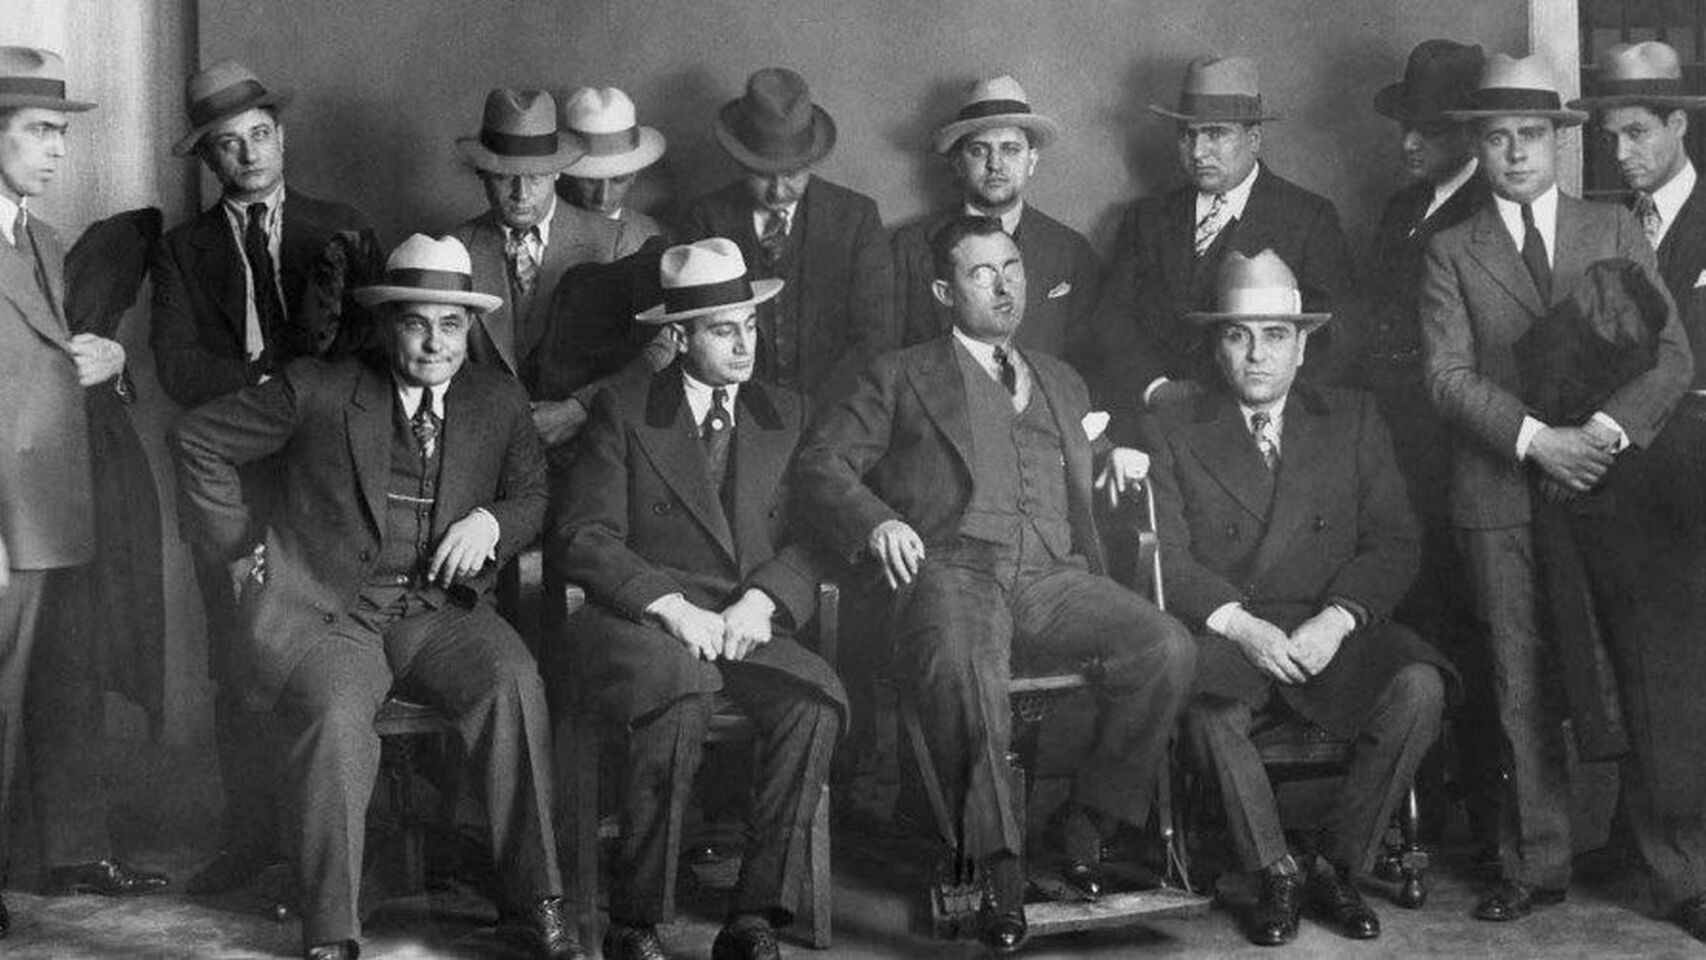
\includegraphics[width = 0.8\textwidth]{img/cosa_nostra}

{\small Cosa Nostra's `The Commission'}

\vspace{20pt}

\begin{itemize}
  \item How does a state resembles a criminal organization?
\end{itemize}

\end{frame}

\begin{frame}
\frametitle{The state as a criminal organization}
\centering

\begin{itemize}
  \item Protection racket: Offering protection (services) in exchange for taxes
  \item Only works if there's territorial monopoly
  \item Use of violence as an enforcing mechanism
\end{itemize}

\end{frame}

\begin{frame}
\frametitle{The state as a criminal organization}
\centering

\begin{minipage}{0.63\textwidth}\centering
\begin{itemize}
\item \textit{Pizzo} in Italy (Mafia in Sicily, 'Ndrangheta in Calabria, Camorra in Campania, etc)
\item Protection money paid by local businesses to a criminal organization
\item If you pay you get access to services: protection, speedy bureaucracy, resolution of conflicts...
\item If you don't pay? Business destroyed
\item Who do you pay? Local organization
\end{itemize}
\end{minipage}\hfill
\begin{minipage}{0.36\textwidth}\centering
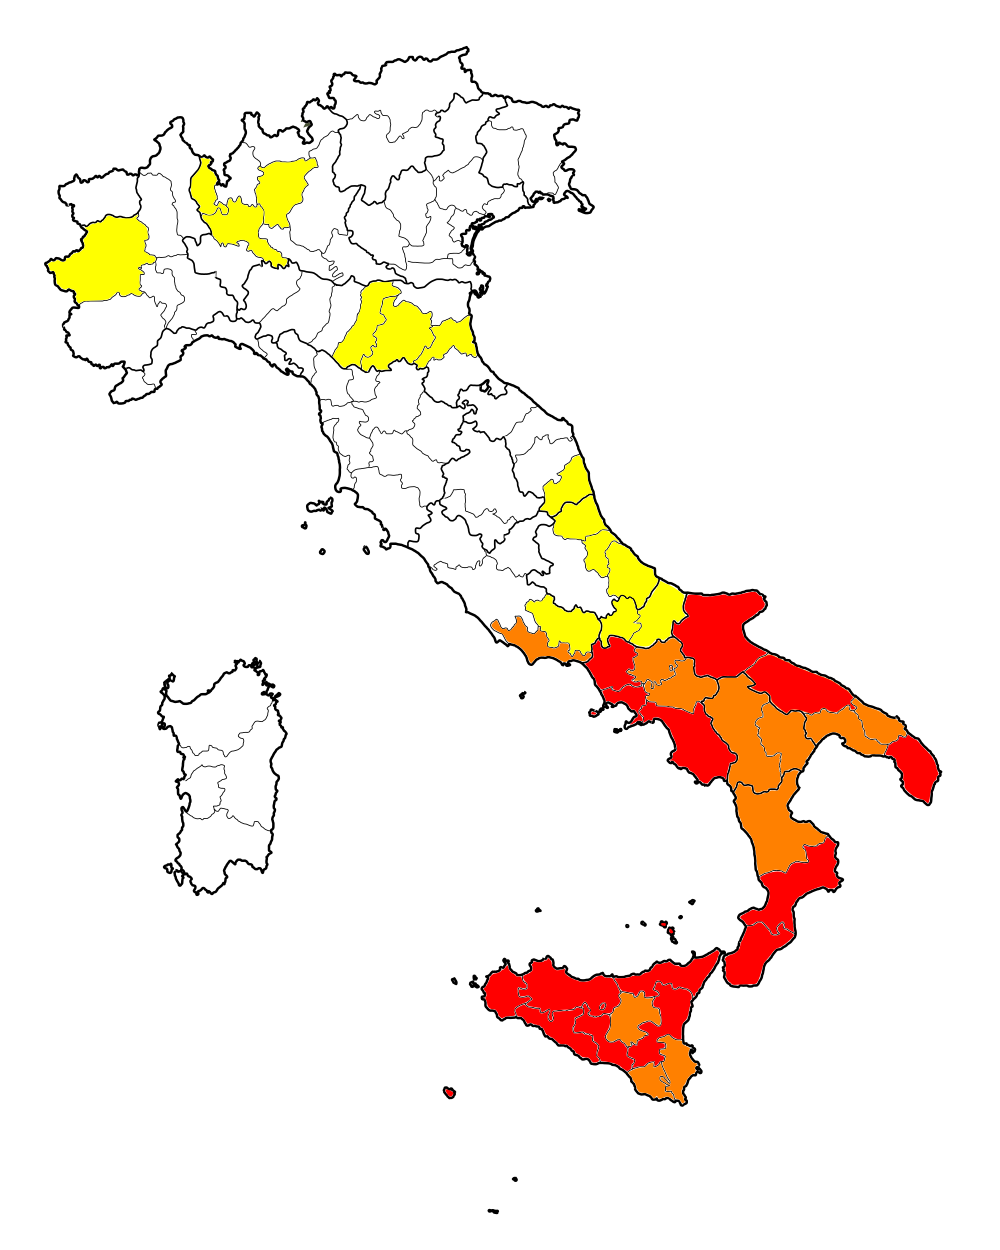
\includegraphics[width = 0.9\textwidth]{img/italy_pizzo}\\
{\small Extortion in Italy, 2008}\\\vspace{5pt}
{\tiny Source: Daygum (Wikipedia),\\data from Confesercenti Survey\\}
\end{minipage}

\end{frame}

\begin{frame}
\frametitle{The state as a criminal organization}
\centering

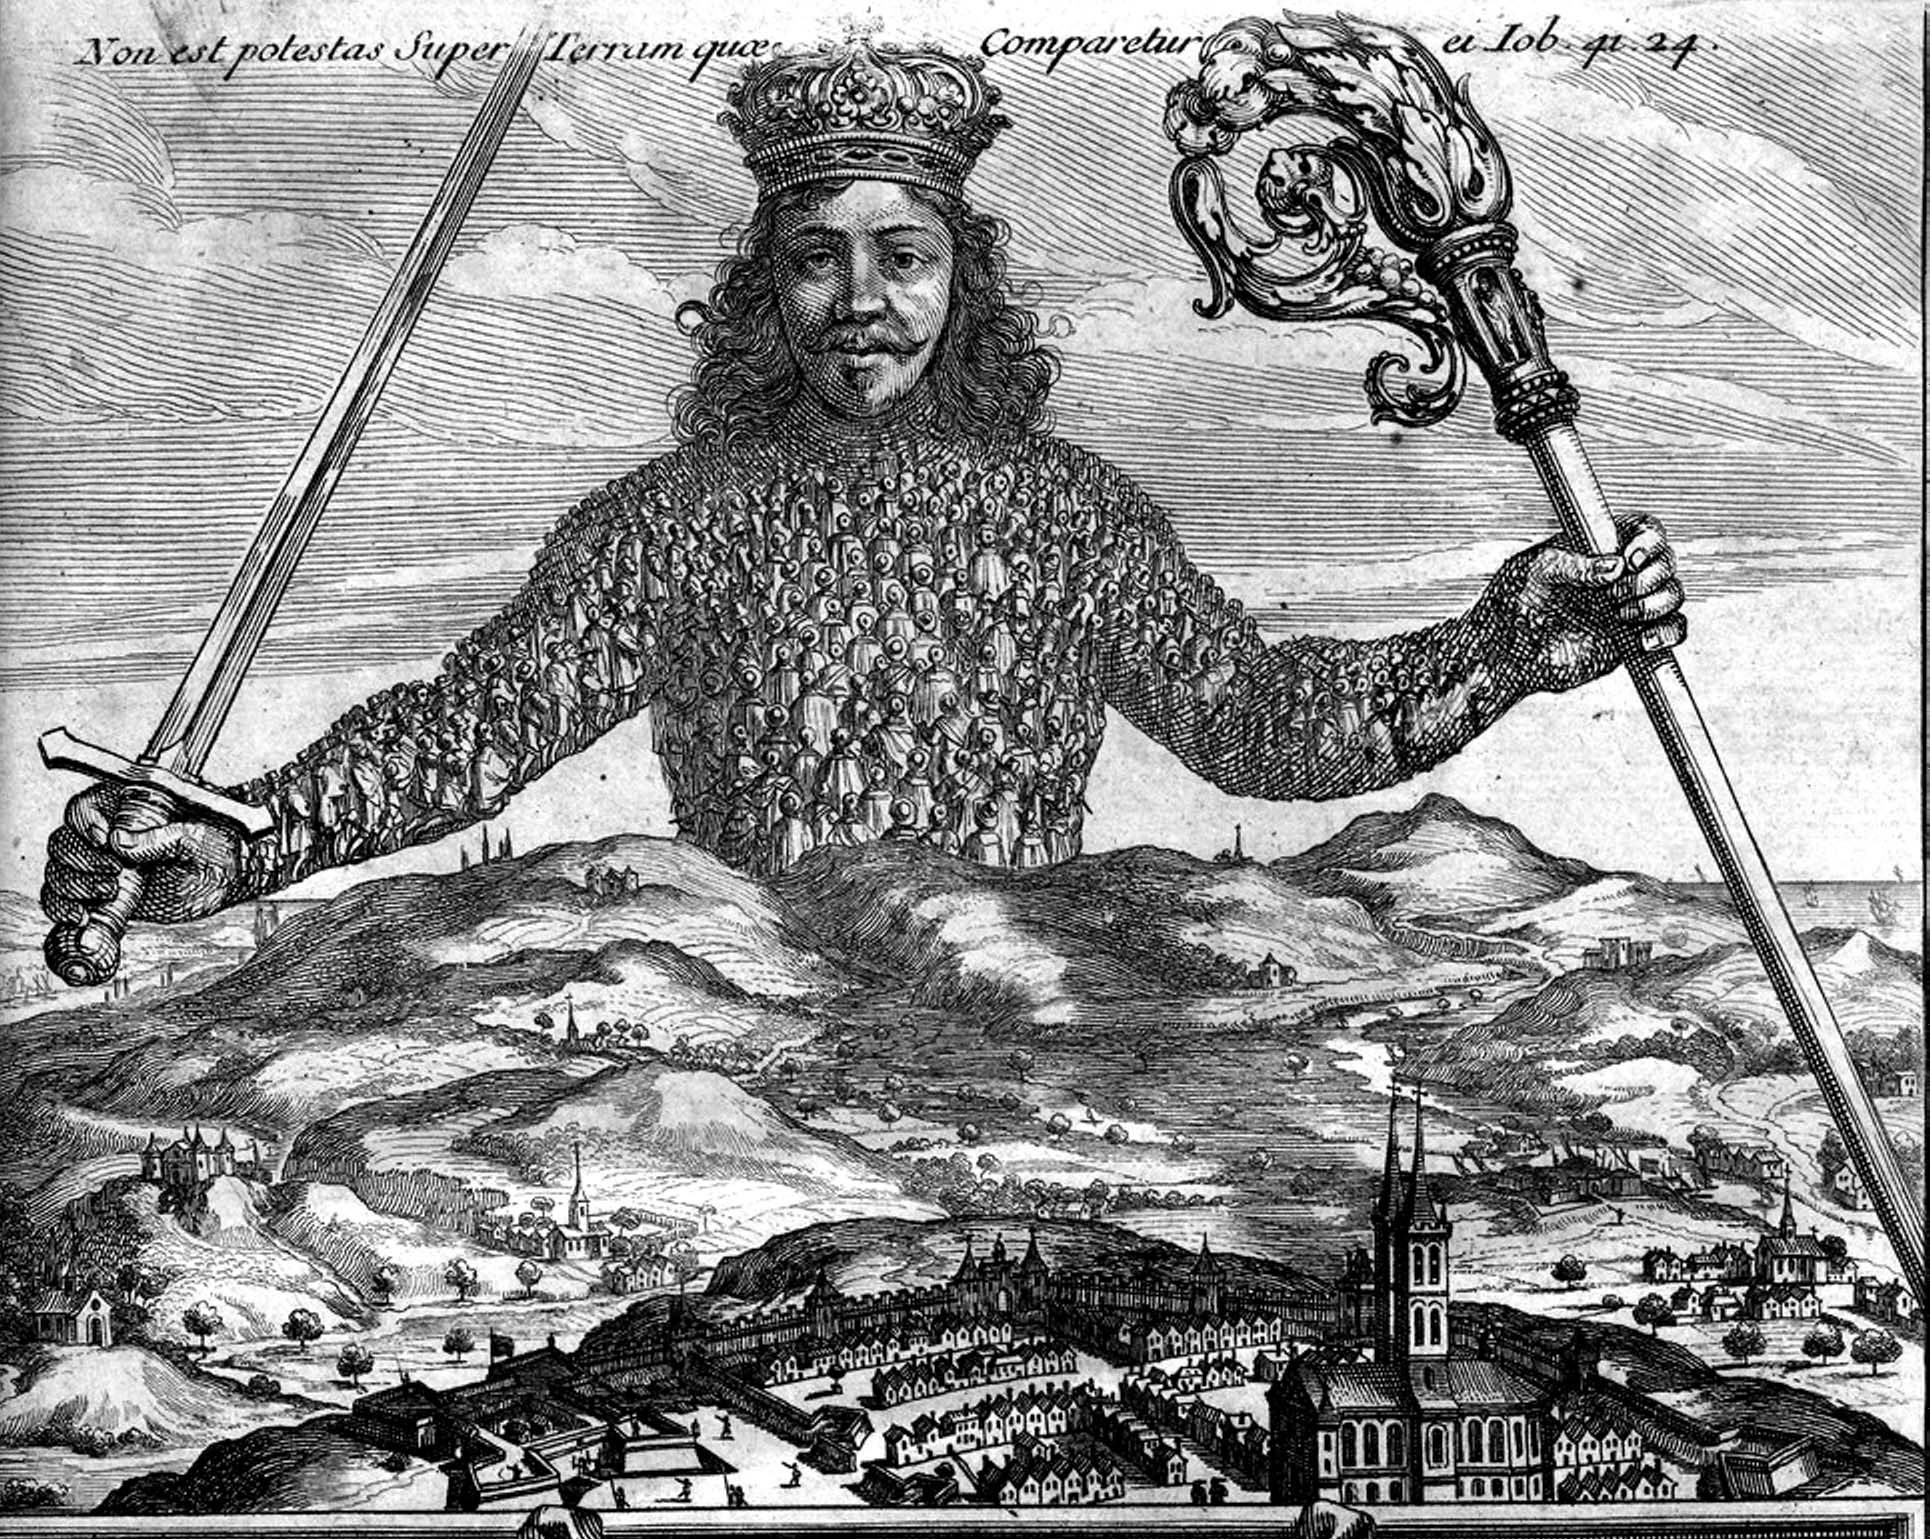
\includegraphics[width = 0.7\textwidth]{img/leviathan}

\vspace{20pt}

{\small Hobbes' \textit{Leviathan}}

\end{frame}


% ----------------------------------------------------
\begin{frame}
\frametitle{The origins of states}
\centering

\begin{itemize}
  \item How did the modern state emerge?
\end{itemize}

\end{frame}
% ----------------------------------------------------

\begin{frame}
\frametitle{Charles Tilly and the origins of European states}
\centering

\begin{minipage}{0.66\textwidth}\centering
\begin{itemize}[<+->]
\item State-formation process in Europe
\item The protection racket idea: kings and rulers were not different from the initial competitors (legitimacy happens afterwards)
\item Dual process of establishing a monopoly of violence and building state institutions
\item ``War made the state and the state made war''
\end{itemize}
\end{minipage}\hfill
\begin{minipage}{0.33\textwidth}\centering
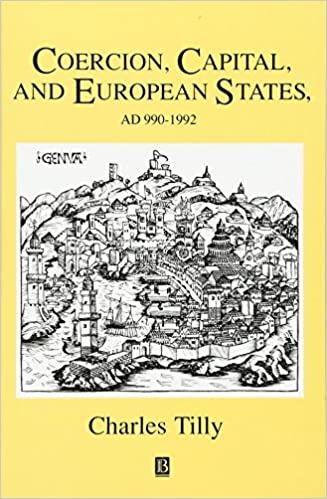
\includegraphics[width = 0.9\textwidth]{img/tilly_book}\\\vspace{5pt}
{\small Charles Tilly (1990)}
\end{minipage}

\end{frame}

\begin{frame}
\frametitle{War-making and state-making in Europe}
\centering

\begin{minipage}{0.49\textwidth}\centering
  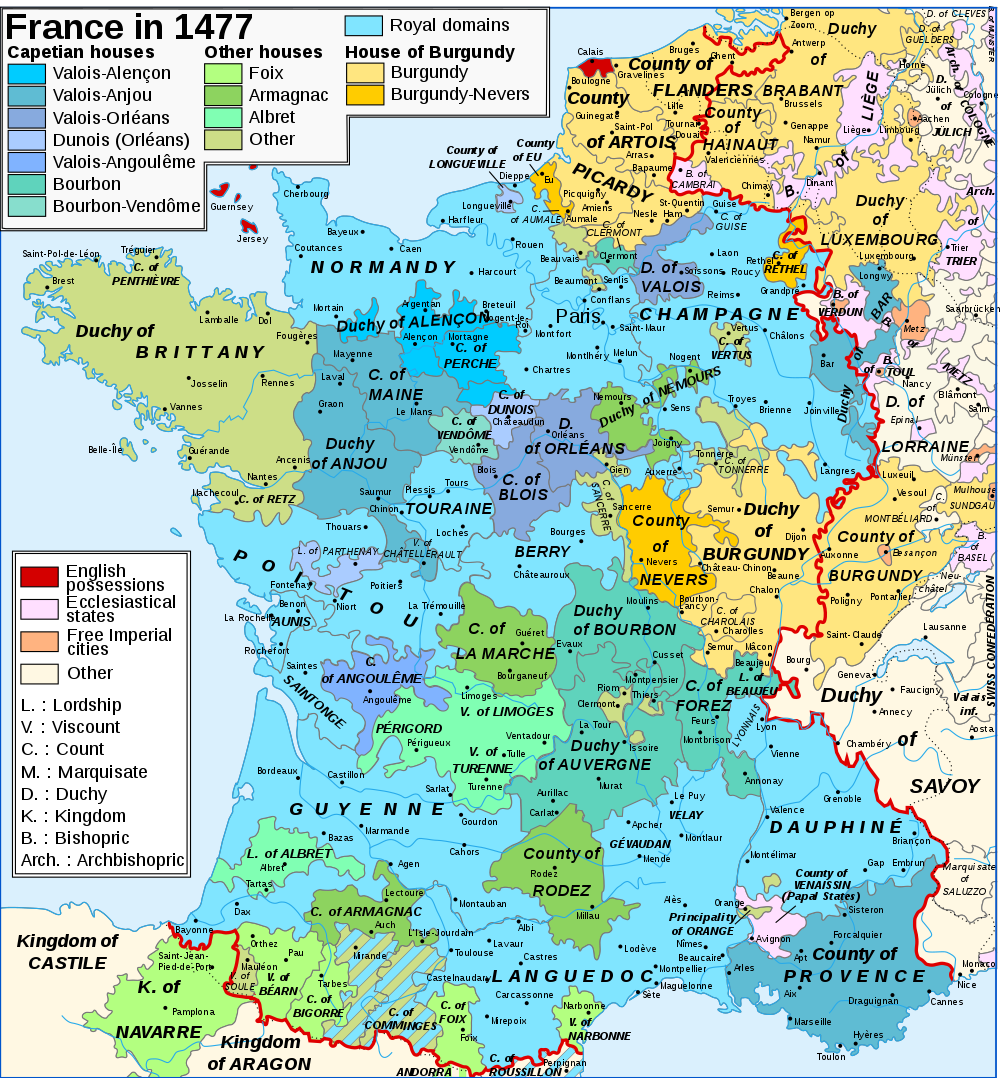
\includegraphics[width = \textwidth]{img/france1477}\\
  {\small France around 1477}
\end{minipage}\hfill
\begin{minipage}{0.49\textwidth}\centering
  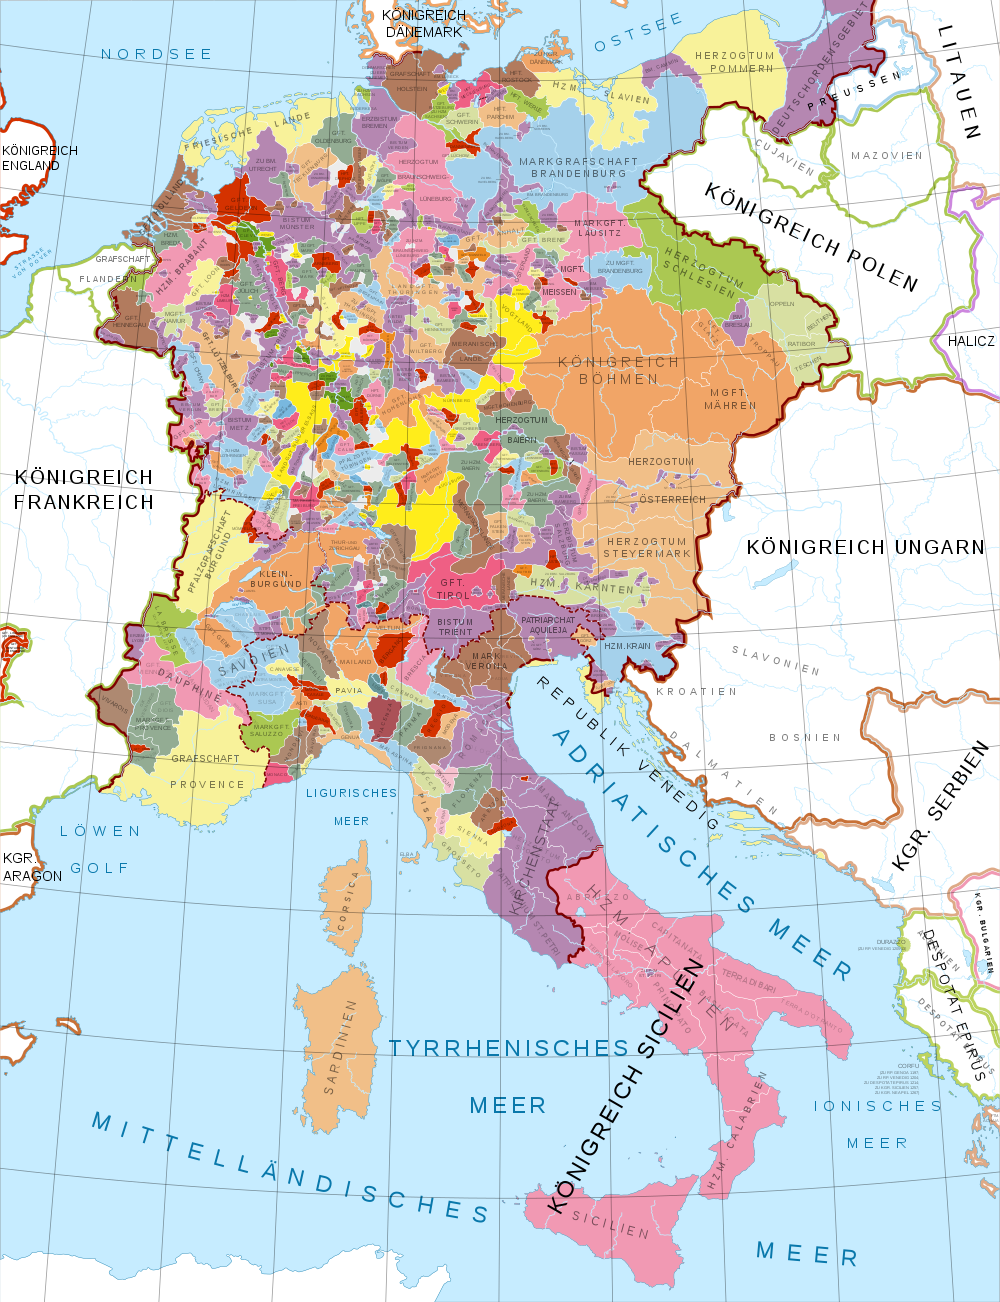
\includegraphics[width = \textwidth]{img/holy_roman_empire_1200}\\
  {\small Holy Roman Empire around 1200}
\end{minipage}

\end{frame}

\begin{frame}
\frametitle{War-making}
\centering

\begin{itemize}[<+->]
\item Setting: early states in Europe competed for territory and power
\item Context of Feudalism: decentralized means of violence, fragmented rule
\item Pressures for war-making: conquer or be conquered
\item Kings or powerful lords did not use \textit{direct rule}, but relied on intermediaries
\begin{itemize}
  \item Direct vs indirect rule
\end{itemize}
\item Innovations in the technology of war changed it all: war became more and more expensive
\end{itemize}

\end{frame}

\begin{frame}
\frametitle{State-making}
\centering

\begin{itemize}[<+->]
\item In the process of waging war against external enemies, two more things happened
\begin{itemize}
  \item Bureaucracy \& internal monopoly
\end{itemize}
\item How do you finance the war? Taxing the population
\item Tax and administration institutions developed
\item The intermediaries in \textit{indirect rule} (feudal lords, etc) were also potential enemies to the king
\item Gaining power among internal threats, establishing monopoly of violence (not always successfully)
\item Later on: censuses, modern bureaucracy, police
\end{itemize}

\end{frame}

\begin{frame}
\frametitle{War-making and state-making}
\centering

\begin{itemize}
\item ``War made the state and the state made war''
\item[]
\item Different from other conceptions of the origins of the state (e.g. social contract)
\item Rooted in security concerns: remember that protection threats (esp. external) is usually the idea of a minimum state
\item ``Love-hate relationship between state makers and pirates or bandits''
\item The service side of the state was developed as a response to population resistance to coercive governance
\end{itemize}

\end{frame}


\begin{frame}
\frametitle{War and the state development process}
\centering

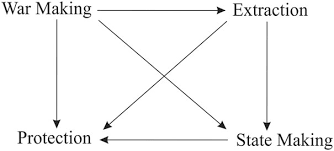
\includegraphics[width = 0.5\textwidth]{img/tilly_causal_chain}

\vspace{20pt}

{\small Tilly's causal chain of European state-making}

\vspace{20pt}

\begin{itemize}
  \item It all starts with war-making: states are a by-product of rulers' efforts to increase the means of war
  \item And it's all about violence: coercive violence is used to develop the monopoly of legitimate violence
\end{itemize}

\end{frame}

\begin{frame}
\frametitle{War-making and state-making}
\centering

\begin{quote}
  By the later eighteenth century, through most of Europe, monarchs controlled permanent, military forces that rivaled those of their neighbors and far exceeded any other organized armed force within their own territories. The state's monopoly of large-scale violence was turning from theory to practice. (Tilly 1985, p. 174)
\end{quote}

\begin{itemize}[<+->]
\item Westphalian international system ``fully developed''
\item Shift to (more costly) direct rule after French Revolution
\item Only possible after kings won previous ``civil wars''
  \begin{itemize}
    \item The development of the police in the 19th century was the latest step, reaching out the most local challengers
  \end{itemize}
\item State-making $\neq$ peace-making
\end{itemize}

\end{frame}

% THE TWO IMPLICATIONS
% -- Popular resistance mattered, because the higher it was, the more concessions state makers had to do (with its later path-dep implications)
% -- The relative balance of the four activities defined the future state


\begin{frame}
\frametitle{Bringing the international system in}
\centering

\begin{itemize}[<+->]
  \item Early on, no distinction between internal and external threats
  \item Later on, war as major moving force of the international system, with similar dynamics as in internal state making (violence)
  \item Peace of Westphalia in 1648: clear borders of sovereignty emerge and after each war, states are re-defined (usually decreasing in number)
  \item If you think about this, the distinction between civil wars and inter-state wars maybe blurs a bit, at least when you look at them from a (European) historically point of view
\end{itemize}

\end{frame}

\begin{frame}
\frametitle{War and state services in the XXth century?}
\centering

\begin{minipage}{0.66\textwidth}\centering
\begin{itemize}
  \item The selection process among states because of warfare does not work anymore
  \item But maybe the logic of offering something in exchange for contributing to the efforts of war does
  \item World War II and mass mobilization led to an increase in tax to the wealthy as compensation
\end{itemize}
\end{minipage}\hfill
\begin{minipage}{0.33\textwidth}\centering
\includegraphics[width = 0.9\textwidth]{img/scheve-stasavage}\\
{\small Kenneth Scheve \& David Stasavage (2016)}
\end{minipage}

\end{frame}

\begin{frame}
\frametitle{Can we generalize from European history?}
\centering

\begin{itemize}[<+->]
  \item Tilly's bellicist theory left one question open:
  \item[] ``The fact that European states formed in a certain way, then imposed their power on the rest of the world, guarantees that non-European experience will be different''
  \item So how or why did it happen outside of Europe?
  \item Also related to the other part of the theory: capital development
\end{itemize}

\end{frame}

\begin{frame}
\frametitle{Can we generalize from European history?}
\centering

\begin{minipage}{0.6\textwidth}\centering
  \begin{itemize}
    \item In Africa, Herbst claimed that absence of international wars explains weak states
    \item Historically low population density, rough terrain: no state emergence
    \item ``Addis rule'' froze borders after decolonization
    \item Problem: there are some disputes (and correlated taxing), and also these states face much more internal than external threats, shouldn't this be an incentive for state-building or work the same way?
  \end{itemize}
\end{minipage}\hfill
\begin{minipage}{0.4\textwidth}\centering
  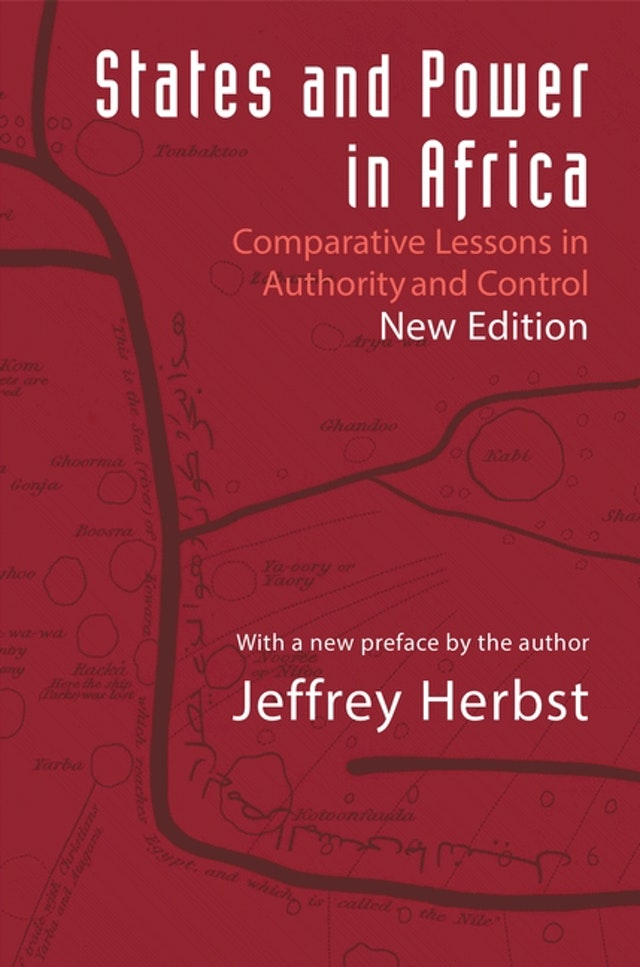
\includegraphics[width = 0.8\textwidth]{img/herbst}\\
  {\small Jeffrey Herbst (2015)}
\end{minipage}

\end{frame}

\begin{frame}
\frametitle{Can we generalize from European history?}
\centering

\begin{itemize}[<+->]
  \item Tilly's theory applied to other regions of the world
  \item Tribute-taking empires in Asia (Victoria Hui, \textit{War and State Formation in Ancient China and Early Modern Europe})
  \item Existence of capital in Latin America (Miguel A Centeno, \textit{Blood and debt: War and the nation-state in Latin America})
  \item[]
  \item One pressing question today is: How should we see internal conflicts? Do they strengthen of weaker state-formation?
\end{itemize}

\end{frame}


% ----------------------------------------------------
\begin{frame}
\frametitle{Generalizing from European history}
\centering

\begin{minipage}{0.6\textwidth}\centering
  \begin{itemize}[<+->]
    \item State formation took place when capitalism, rather than war, ruled internationally
    \item Because of pursuing benefits of trade, Latin American countries created weak states, with patrimonial structures, etc
    \item \textbf{State formation} (monopoly of violence within delimited borders) vs \textbf{state building} (switch from patrimonial to bureaucratic administration)
    \begin{itemize}
      \item Which can happen at the same time (Europe), or not
    \end{itemize}
  \end{itemize}
\end{minipage}\hfill
\begin{minipage}{0.4\textwidth}\centering
  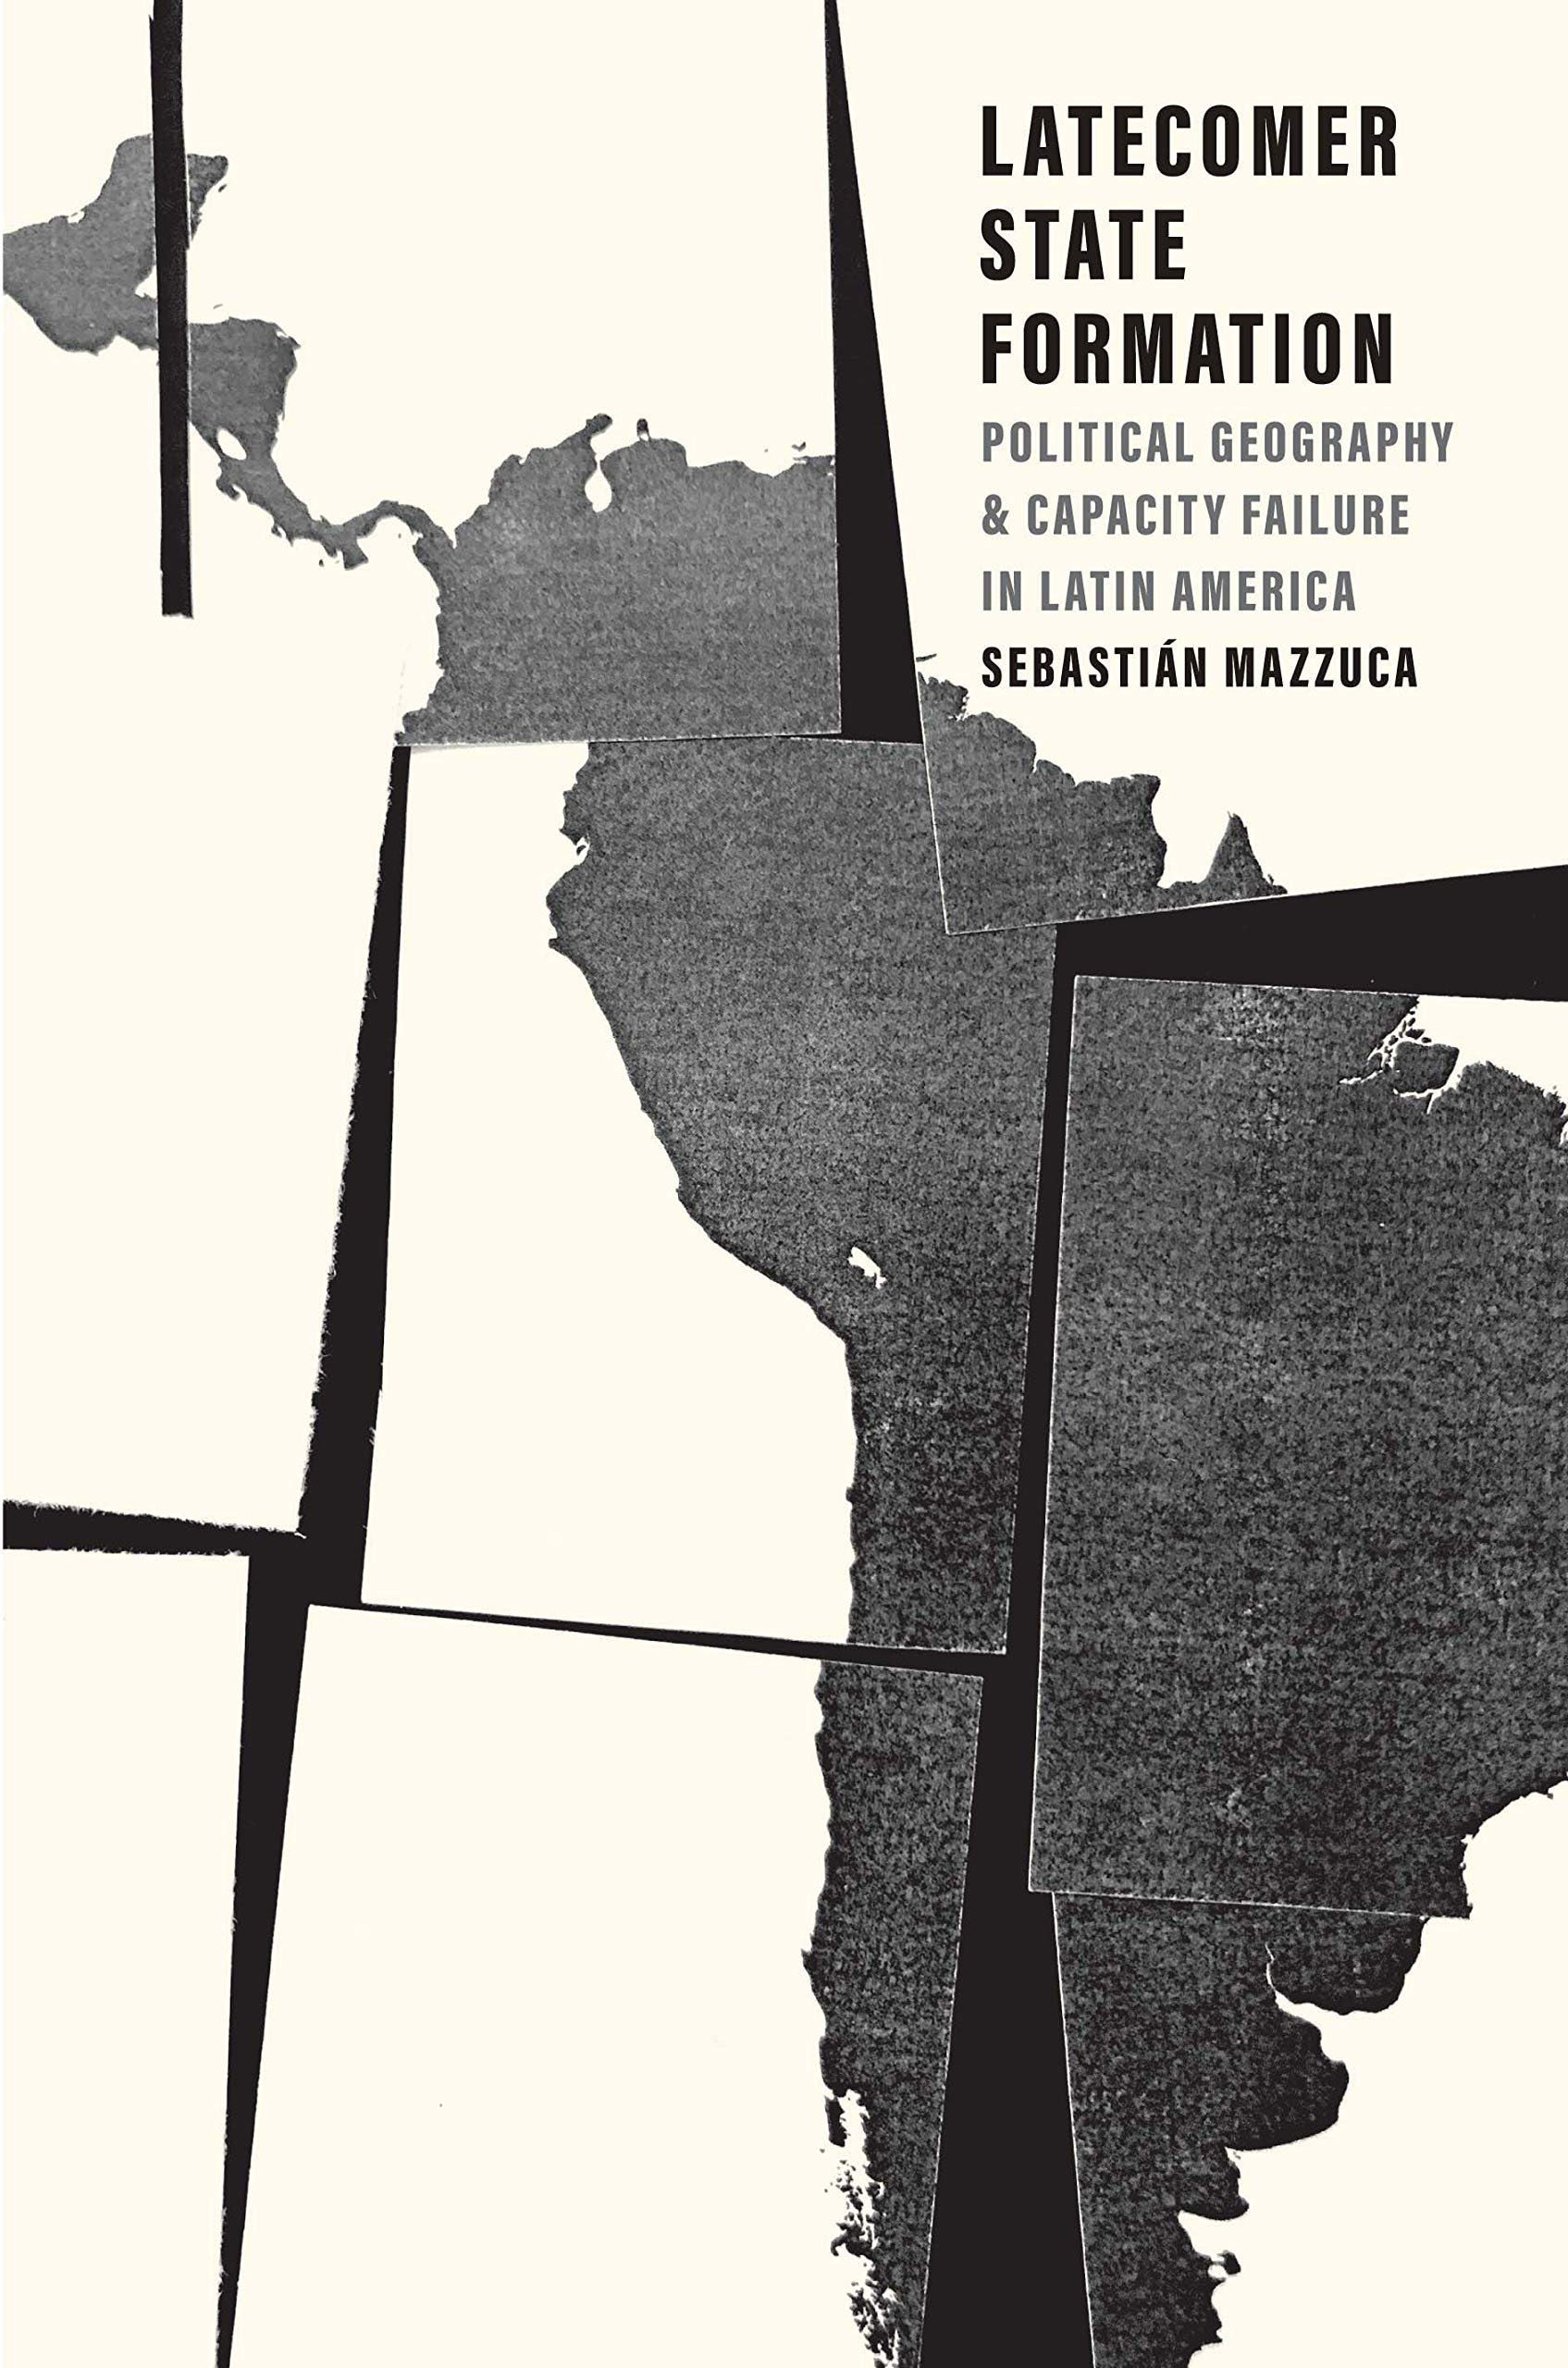
\includegraphics[width = 0.8\textwidth]{img/mazzuca_book}\\
  {\small Mazzuca (2021)}
\end{minipage}

\end{frame}
% ----------------------------------------------------

% ----------------------------------------------------
\begin{frame}
\frametitle{Generalizing from European history}
\centering

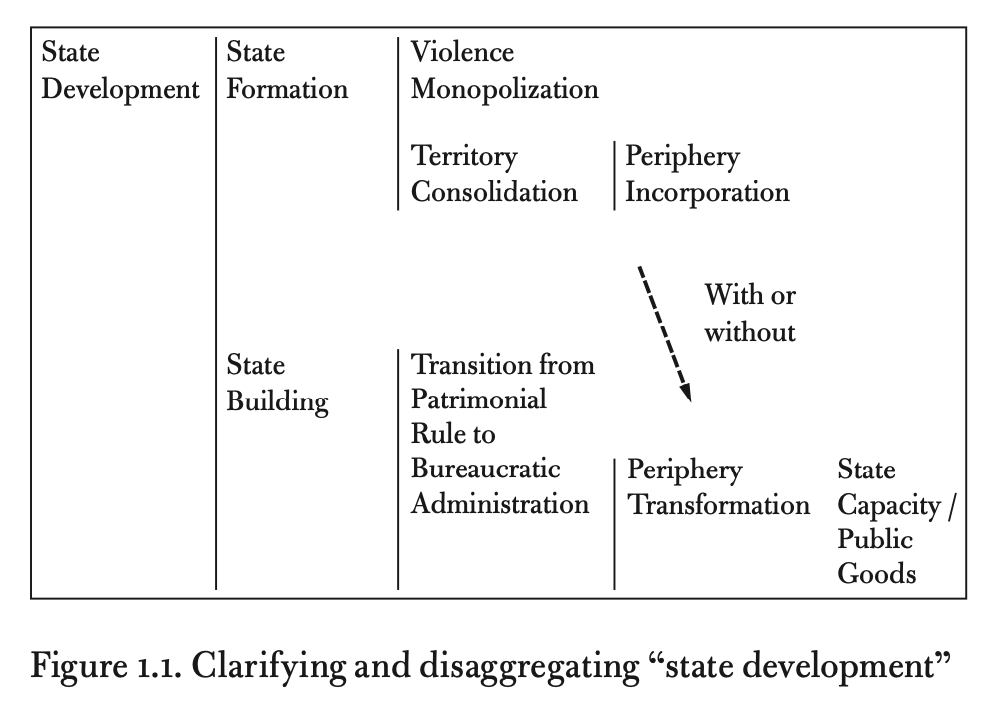
\includegraphics[width = 0.75\textwidth]{img/mazzuca_table1}

\end{frame}
% ----------------------------------------------------

% ----------------------------------------------------
\begin{frame}
\frametitle{Generalizing from European history}
\centering

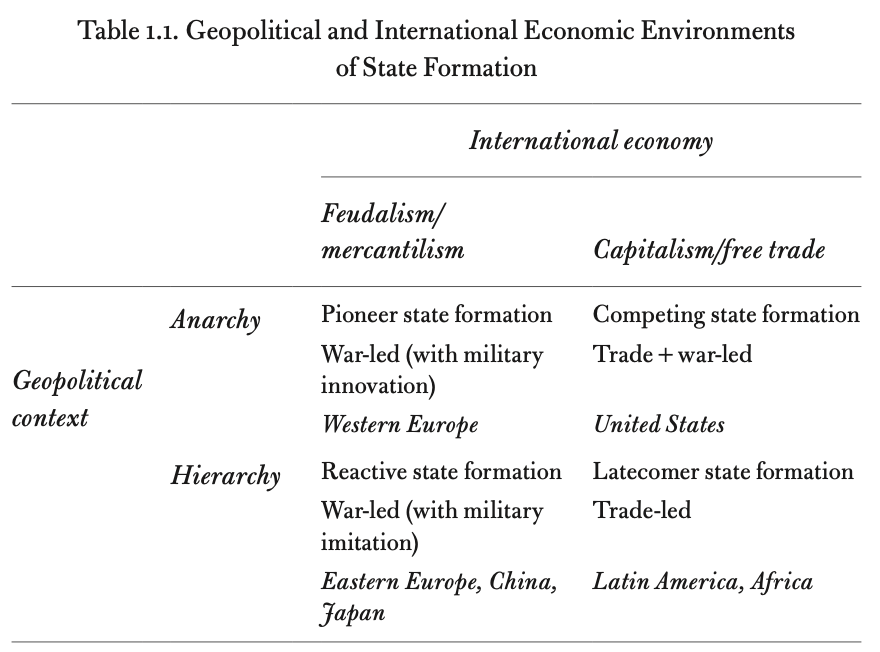
\includegraphics[width = 0.75\textwidth]{img/mazzuca_table2}

\end{frame}
% ----------------------------------------------------


\begin{frame}
\frametitle{Two critiques to the bellicist theory}
\centering

\begin{itemize}
  \only<1>{\item European system environment is not exogenous}
  \only<1>{\item Why were so many independent states in Europe fighting each other? Not random, it needs to be explained}
  \only<1>{\item Failure of other systems (empire, theocracy): tribute-taking empires in Asia, scarcity of states in Africa}
  \only<2>{\item Which micro-level mechanisms explain that war-making increases state capacity?}
  \only<2>{\item States can increase internal capacity, but can also look for allies, bandwagon on stronger powers, etc}
  \only<2>{\item In other words, it does \textit{not} always happens this way, fighting could also lead to   chaos and state collapse, and external threats do not necessarily lead to stronger states}
  \item[]
  \item[] {\small \textit{See}: Hendrik Spruyt in \textit{Does War Make States?} (CUP, 2017)}
\end{itemize}

\end{frame}

\begin{frame}
\frametitle{The role of legitimacy}
\centering

\begin{itemize}[<+->]
  \item So are states really like criminal protection rackets?
  \item Tilly's account assumes so: at the beginning, there were many competing authorities offering protection and kings were just the better providers of protection and thus manage to rule above them all
  \item But legitimacy could have played a role: maybe people did care about who ended up ruling over all
  \item Kings were not exactly the same as minor feudal lords: the could claim legitimacy and loyalty, and emerge as the ultimate defenders from `outside' threats
  \item Think of situations of fragmented rule without cultural unity: e.g. warlords in Somalia
  \begin{itemize}
    \item (Even though we cannot talk about nationalism in Early Modern Europe)
  \end{itemize}
\end{itemize}

% check last paragraph of Tilly 1985!
\end{frame}

\begin{frame}
\frametitle{What is this all about}
\centering

\begin{itemize}[<+->]
  \item War and violence and the state are deeply related from the start
  \item Coercion and the monopoly of violence still define many if not all problems of political order today
  \item Very relevant questions for contexts of civil wars or state collapse: Somalia, DRC
  \item Do preferences for centralized or decentralized force matter?
  \begin{itemize}[<+->]
    \item War and state formation in multi-ethnic countries?
    \item Why Mafia flourished in southern Italy? And why do we see higher mobilization against it today? (\textit{Addiopizzo} movement)
  \end{itemize}
\end{itemize}

\end{frame}


\begin{frame}
\frametitle{Empirical evidence}
\centering

\begin{minipage}{0.6\textwidth}\centering
  \begin{itemize}
    \item States created statistics, so it's difficult to study its formation empirically
    % \item Sánchez de la Sierra (2020) ``On the Origins of the State: Stationary Bandits and Taxation in Eastern Congo'' (\textit{Journal of Political Economy})
    \item How do `stationary bandits' emerge?
    \item Studying eastern DRC, and exploiting price of coltan and gold
    \item When coltan price goes up, rebel groups establish monopoly of violence in mines
    \item When gold price goes up, rebel groups establish taxing mechanisms in villages
  \end{itemize}
\end{minipage}\hfill
\begin{minipage}{0.39\textwidth}\centering
  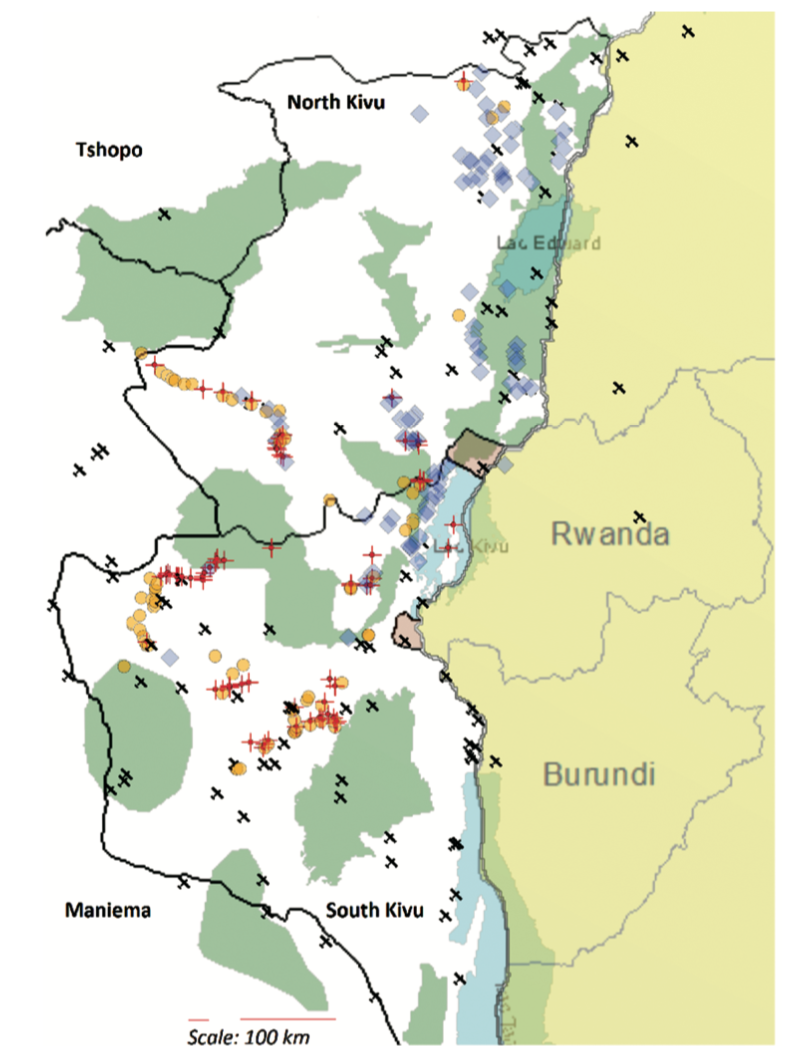
\includegraphics[width = \textwidth]{img/sanchez_de_la_sierra_sample}\\
  {\footnotesize Sánchez de la Sierra (2020)\\\textit{Journal of Political Economy}\\}
\end{minipage}

\end{frame}

\begin{frame}
\frametitle{James C. Scott on the origin of state}
\centering

\begin{minipage}{0.6\textwidth}\centering
  \begin{itemize}
    \item Against the usual idea that people freely chose to settle and form states
    \item The origin of the state matched with violent coercion, diseases, and slavery
    \item States `domesticated' humans as much as they domesticated animals
    \item Chapter 5: role of war and violence in the gathering of population
  \end{itemize}
\end{minipage}\hfill
\begin{minipage}{0.39\textwidth}\centering
  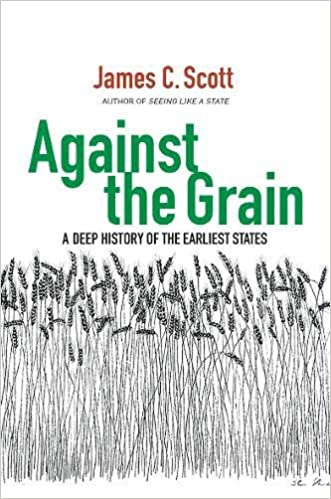
\includegraphics[width = 0.9\textwidth]{img/scott_against}\\
  James C. Scott (2017)
\end{minipage}

\end{frame}

% ----------------------------------------------------
\begin{frame}
\frametitle{What about actual gangs?}
\centering

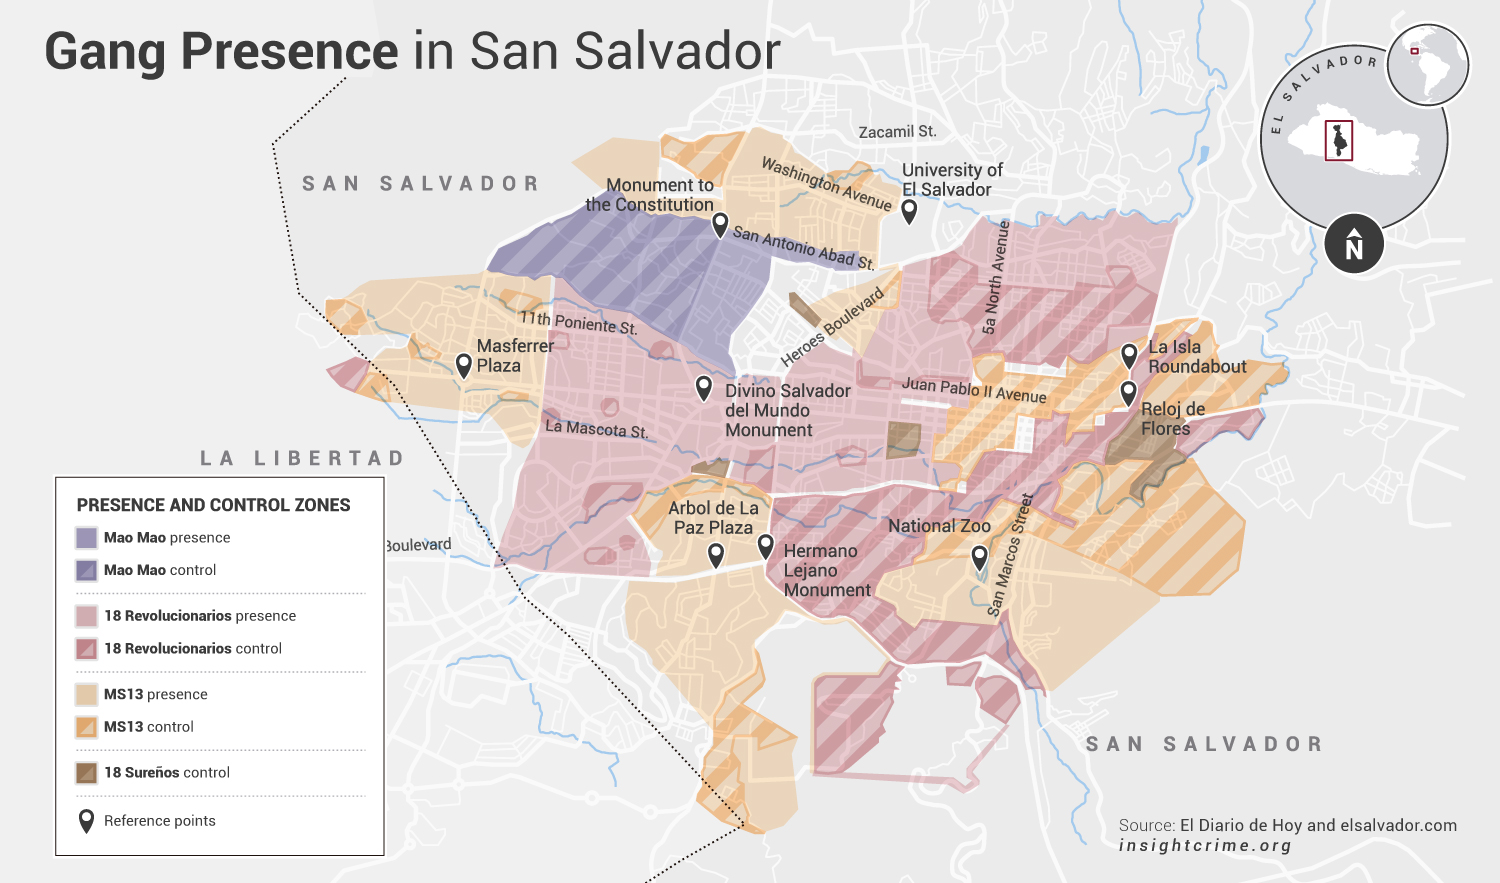
\includegraphics[width = \textwidth]{img/gangs_salvador}

\end{frame}
% ----------------------------------------------------


\begin{frame}
\frametitle{.}
\centering

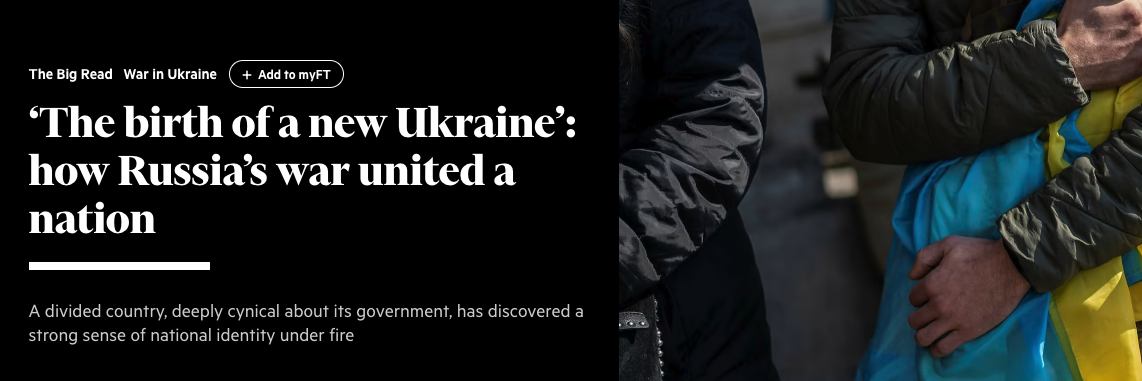
\includegraphics[width = \textwidth]{img/ft}

\end{frame}

\end{document}
